\chapter{Krav} \label{Krav}
I dette afsnit beskrives hvilke krav der er stillet til det endelige produkt. I krave indgår både krav opstillet af institutionen IHA, egne krav i udarbejdet i forbindelse med kravspecifikationen  (\textit Se dokumentationen afsnit ...) 
\section{IHA krav}
Fra IHA’s side er der på forhånd defineret nogle krav til projektets indhold, hvilket indebærer:\\ \\
Software 
\begin{itemize}
	\item Programmet skal programmeres i C\#
	\item Programmet skal kunne kalibrerer blodtrykssignalet og foretage en nulpunktsjustering
	\item Programmet skal kunne vise blodtrykssignalet kontinuert
	\item Programmet skal kunne lagre de måte data i enten en tekstfil eller en database
	\item Programmet skal kunne filtrerer blodtrykket i selve programmet via et digitalt filter, dette skal kunne slås til og fra
\end{itemize}

Hardware
\begin{itemize}
	\item Der skal designes et aktivt 2. ordens lavpasfilter af typen Sallen-Key med unity gain
	\item Filteret skal designes som et Butterworth filter med cut off frekvens på 50 Hz. C2 skal vælges til 680 nF og R1 = R2. Operationsforstærkeren skal være af typen OP27
\end{itemize}

\section{Funktionelle krav}
Disse opstillede krav indgår i enten Use cases eller ikke-funktionelle krav, med vurderingen "must". De funktionelle krav er udformet som use cases, hvor følgende 6 use cases (figur \ref{UC diagram}) er valgt:

\begin{figure}[H]
	\centering
	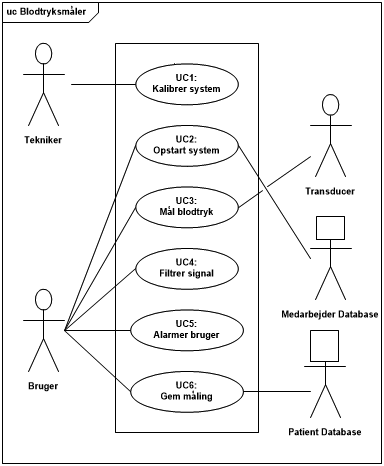
\includegraphics[width=0.8\textwidth]{Figurer/ISE/UcDiagram2}
	\caption{Use case diagram}
	\label{UC diagram}
\end{figure}

\textbf{Kalibrer system}\\
Use casen "Kalibrer system"\ beskriver hvordan systemet kalibreres af en tekniker, hvilket sørger for en mere præcis blodtryksmåling.\\[1ex]
\textbf{Opstart system}\\
Use casen "Opstart system"\ beskriver hvordan brugeren logger ind i systemet samt nulpunktsjusterer systemet. Brugeren logger ind i systemet ved at indtaste brugernavn og kode hvorved log ind oplysningerne tjekkes i medarbejder databasen. Herefter vælger brugeren at nulpunktsjusterer systemet hvorefter systemet starter.\\[1ex]
\textbf{Mål blodtryk}\\
Use casen "Mål blodtryk"\ beskriver hvordan blodtrykket startes og vises i brugergrænsefladen, her vises både det systoliske- og diastoliske blodtryk samt pulsen.\\[1ex]
\textbf{Filtrer signal}\\
Use casen "Filtrer signal"\ beskriver hvordan brugeren har mulighed for at til- og fravælge et digitalt filter.\\[1ex]
\textbf{Alarmer bruger}\\
Use casen "Alarmer bruger"\ beskriver hvordan systemet i tilfælde af for højt eller lavt blodtryk kan alarmere brugeren. Yderlige er kan brugeren justere grænseværdierne for alarmer, samt udskyde denne.\\[1ex]
\textbf{Gem måling}\\
Use casen "Gem måling"\ beskriver hvordan brugeren kan gemme og afslutte en måling. Her indtastes patientens CPR nr også.

\section{Ikke-funktionelle krav}
De ikke-funktionelle krav er opstillet på baggrund af FURPS+, en model for klassifikation af krav. Yderligere er vigtigheden af hvert enkelt krav vurderet ved MoSCoW, hvor de vigtigste, kategorien must, er listet her:

\begin{enumerate}
	\item (M) Brugeren skal kunne starte en ny måling indenfor XX sekunder efter opstart af programmet 
	\item (M) Systemet skal kunne foretage en nulpunktsjustering
	\item (M) Systemet skal kunne forstærke signalet fra transduceren ca. 400 gange +/- 10\%
	\item (M) Systemet skal kunne filtrere signalet med det indbyggede analoge antialiaserings filter med en båndbredde på 50 Hz, samt en cutoff frekvens på 50 Hz
	\item (M) Programmet skal kunne vise blodtrykket som funktion af tiden
\end{enumerate}



